\RequirePackage[l2tabu, orthodox]{nag}
%
    % http://www.tug.org/texlive/Contents/live/texmf-dist/doc/latex/nag/nag.pdf
    % Check for many common mistakes, and give hints on what to use instead.
    % However, always refer to l2tabu for more detailed explanations.
    % Orthodox checks for pitfalls that are not technically incorrect.
    % If you know what you’re doing, omit orthodox.

\documentclass[12pt,a4paper,british]{article}
\usepackage{etex}
\usepackage{mathptmx}
% \renewcommand{\familydefault}{\rmdefault}
\usepackage[T1]{fontenc}
\usepackage[latin9]{inputenc}
% \usepackage{lmodern}
\usepackage{mathpazo}
\usepackage[protrusion=true,expansion]{microtype}
\usepackage{color,xcolor}
\usepackage{verbatim}
\usepackage{enumitem}
\usepackage{amsmath,amsthm,amsfonts,mathrsfs,bm,mathtools}
\usepackage{graphicx}
\usepackage[a4paper, margin=1.1in]{geometry}
%\geometry{verbose,tmargin=3cm,bmargin=3cm,lmargin=2.5cm,rmargin=2.5cm}
\usepackage{prettyref}
\usepackage[authoryear]{natbib}
\usepackage{booktabs,multirow,multicol,rccol}
\usepackage{subfig}
\usepackage{eurosym}
\usepackage{babel}

%############# tikz ######################
\usepackage{tikz}
\usepackage{svg}
\tikzset{every picture/.style={line width=0.75pt}} %set default line width to 0.75pt

\DeclareMathOperator*{\maxi}{maximize}

\usepackage{todonotes}
    % Use the option "disable" to suppress notes
    % use \missingfigure to locate a place holder for a figure
    % \missingfigure{} has optional text to add
%############# tikz ######################

\usepackage[unicode=true,
			bookmarks=true,
			bookmarksnumbered=true,
			bookmarksopen=false,
			breaklinks=false,
			pdfborder={0 0 1},
			backref=false,
			colorlinks=true]{hyperref}
\hypersetup{final,
			bookmarksopen,
			bookmarksnumbered,
			urlcolor={blue},
			linkcolor={blue},
			citecolor={blue},
			pdfstartview={XYZ null null fitH}}
\pdfminorversion=4
\usepackage{setspace}
\PassOptionsToPackage{nodisplayskipstretch}{setspace}
\onehalfspacing

\ifx\proof\undefined\
  \newenvironment{proof}[1][\proofname]{\par
    \normalfont\topsep6\p@\@plus6\p@\relax
    \trivlist
    \itemindent\parindent
    \item[\hskip\labelsep
          \scshape
      #1]\ignorespaces
  }{%
    \endtrivlist\@endpefalse
  }
  \providecommand{\proofname}{Proof}
\fi


\newlist{casenv}{enumerate}{4}
\setlist[casenv]{leftmargin=*,align=left,widest={iiii}}
\setlist[casenv,1]{label={{\itshape\ \casename} \arabic*.},ref=\arabic*}
\setlist[casenv,2]{label={{\itshape\ \casename} \roman*.},ref=\roman*}
\setlist[casenv,3]{label={{\itshape\ \casename\ \alph*.}},ref=\alph*}
\setlist[casenv,4]{label={{\itshape\ \casename} \arabic*.},ref=\arabic*}

\makeatletter

\providecommand{\casename}{Case}

%%%%%% Theorem env with within section counter %%%%%%
\newtheorem{theorem}{Theorem}[section]
\newtheorem{definition}{Definition}[section]
\newtheorem{assumption}{Assumption}[section]
\newtheorem{prop}{Proposition}[section]
\newtheorem{lemma}{Lemma}[section]

\graphicspath{{graphs/}}


\begin{document}
\title{Allocation and the values of travel time and reliability with automated cars}

\author{Dereje Abegaz \and Mogens Fosgerau}

\date{\today}

\maketitle

\begin{abstract}
Self-driving cars make it increasingly possible to carry out some activities while travelling. This paper analyses a commuter's optimal allocation of total time among different activities and the implication of increased productivity of in-vehicle time on the values of travel time and reliability.
\end{abstract}

\section{Introduction}
\label{sec:introduction}
% by making travel more convenient, more comfortable, or by providing the opportunity to undertake useful economic activity or pleasurable social activity.

% IFT discussion paper [value-saving-travel-time]

In a round-table discussion at ITF, 30 experts from 14 countries identified one of the challenges in the valuation of travel time savings as being the need to account for the quality of travel conditions: The quality component of travel time needs to be incorporated in assessment of the benefits of quicker journey times. The factors that affect the quality of the travel experience include comfort, convenience, frequency, reliability and the possibilities for utilisation of time spent travelling on other activities. In practical terms this means assessing the willingness-to-pay for reduced travel time versus the willingness-to-pay for improvements in travel conditions, and integrating these two assessments in project choice functions (\href{https://www.itf-oecd.org/sites/default/files/docs/value-saving-travel-time.pdf}{Source})

Continued improvements in Information Communication Technology (ITC) and automation, productive use of time ....

Mobile communication devices are transforming the experience of travel, making it possible to work, play games or watch videos while travelling on planes, trains and buses. The car industry promises to free car drivers from driving, thereby enabling an even more drastic transformation of car travel. This paper explores the observation that the new technologies have in common that they make it possible to carry out activities while travelling that substitute for activities elsewhere, at home or at work.

In-vehicle productivity increases when it becomes possible to do things while travelling that were not possible before. This has happened for passengers in trains and buses, who now can use mobile devices  to do new things. It is happening also in planes where internet access during flight is gradually becoming available. Of course, car manufacturers are promising that soon car drivers can be relieved from driving.

This paper looks at the impact of increasing in-vehicle productivity on allocation of commuter's time across different activities and the values of time and reliability. This is of fundamental importance in transport economics and modelling. The values of travel time and reliability are important behavioural quantities as they represent the lion's share of benefits from large infrastructure projects.

We built a model that examines how a commuter optimally allocates his/her time budget among different a activities where some of these activities can only be carried out at home or work. We showed existence of an optimal allocation of time and analysed the optimal scheduling choice in the presence of deterministic and random travel times. We also examined how the values of travel time and reliability change with increasing productivity of in-vehicle time.

Non-work related may include talking on the phone, reading and writing, eating and drinking, planning things, looking through the window, relaxing, watching videos, and work related activities include writing, reading, talking on the phone, planning, video conferencing, etc.

The rest of the paper is organised as follows. The next section sets out the model set up and foundation for the rest of the paper. The third and fourth sections analyse the optimal allocation of time among different activities and the value of travel time, value of reliability and value of headway when trip duration is random or deterministic. The final section provides a summary of our findings and concluding remarks.

\section{The model}
\label{sec:model1}

Consider a commuter who begins a day at home and who has to take a trip to a workplace where he finishes the day. The commuter has a time budget of $Q$ time units on the clock interval $[0, Q]$ and intends to allocate this among different activities. We distinguish three set of leisure and work activities based on whether they can be undertaken at home, at work, or in-vehicle. The first set of work and leisure activities are those which the commuter can carry out at home, at work and while travelling. We call these activities \textit{mobile activities}. While the range of activities that can be performed during a trip depends on the degree of automation of the vehicle, it may include talking on the phone, reading and writing, eating and drinking, planning, relaxing, watching videos, etc. The set of other leisure (resp. work) activities that can only be carried out at home (work) are referred to as \emph{home-based activities} (\emph{work-based activities}). While home-based activities include spending time with relatives and family, cooking and tidying up, work-based activities may include physical meetings, teaching, conducting laboratory experiments, building, etc.


Let $0<T<Q$ be the travel time for the commute trip. Setting aside $T$ units of time for the trip, the commuter has suppose $Q-T$ units of time available which he can freely allocate among the three activities. We denote by $t_{h}$ and $t_{w}$ the time assigned to the home-based and work-based activities, respectively, such that $0<t_{h}\leq t_{d}$ and $0<t_{w}\leq Q-t_{d}-T$ where $t_d$ is the departure time for the commute trip. Given this,  $T+\left(t_{d}-t_{h}\right)+\left(Q-t_{d}-T-t_{w}\right)$ units of time will be available to carry out the mobile activities.


The commuter has preferences over outcomes from the three activities, and given those preferences, he allocates the total time so as to obtain the best result among those available. Suppose a unit of output is produced per unit of time assigned to the home-based or work-based activities while the productivity of time assigned to the mobile activities depends on whether they are undertaken at home, at work, or in-vehicle. Suppose the commuter is fully productive when performing the mobile activity at home or at work but may be less so while travelling. This is controlled by a factor $\alpha \in \left[0, 1\right]$, such that the amount of output per unit time spent in performing the mobile activity is $t_{m} = Q - \left( 1 - \alpha \right) T - t_{h} - t_{w}$. The parameter $\alpha$ indicates the productivity of in-vehicle time relative to time at work or at home.

 \begin{figure}[ht!]
     \centering
     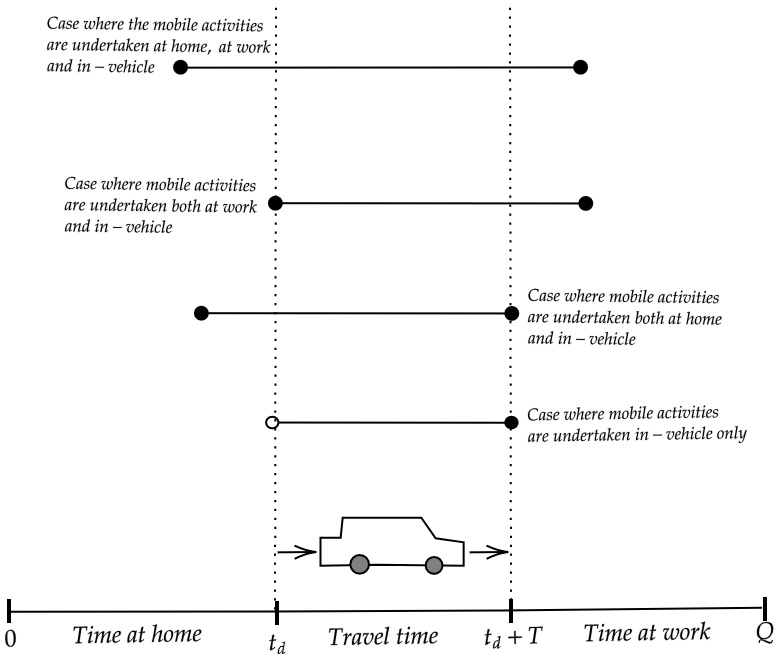
\includegraphics[width=0.5\textheight]{allocationPossibilities.png}
     \caption{Allocation of time with and without binding constraints}
     \label{fig:time_allocation}
 \end{figure}


%% \tikzset{every picture/.style={line width=0.75pt}} %set default line width to 0.75pt       
\begin{tikzpicture}[x=0.75pt,y=0.75pt,yscale=-1,xscale=1, scale=1.1]
%uncomment if require: \path (0,262); %set diagram left start at 0, and has height of 262

%Shape: Brace [id:dp6169517089591515] 
\draw  [line width=1.5]  (78.5,46) .. controls (78.5,41.33) and (76.17,39) .. (71.5,39) -- (55.82,39) .. controls (49.15,39) and (45.82,36.67) .. (45.82,32) .. controls (45.82,36.67) and (42.49,39) .. (35.82,39)(38.82,39) -- (18.5,39) .. controls (13.83,39) and (11.5,41.33) .. (11.5,46) ;
%Shape: Brace [id:dp4131205777115946] 
\draw  [line width=1.5]  (243.5,46) .. controls (243.5,41.33) and (241.17,39) .. (236.5,39) -- (216.75,39) .. controls (210.08,39) and (206.75,36.67) .. (206.75,32) .. controls (206.75,36.67) and (203.42,39) .. (196.75,39)(199.75,39) -- (177,39) .. controls (172.33,39) and (170,41.33) .. (170,46) ;
%Straight Lines [id:da38667449766519557] 
\draw [color={rgb, 255:red, 0; green, 0; blue, 0 }  ,draw opacity=1 ][line width=0.75]    (244,55) -- (229.5,55) -- (225,48) -- (224.5,63) -- (219.5,48) -- (217.5,63) -- (214.5,55) -- (39.5,57) -- (35.5,49) -- (34.5,65) -- (29.5,49) -- (27.5,64) -- (25.5,57) -- (14,57) ;


%Straight Lines [id:da7437120864039053] 
\draw [line width=2.25]    (13,50) -- (13,62) ;


%Straight Lines [id:da34292863475953517] 
\draw [line width=2.25]    (81,50) -- (81,62) ;


%Straight Lines [id:da21717714518989284] 
\draw [line width=2.25]    (169,50) -- (169,62) ;


%Straight Lines [id:da8184808038203972] 
\draw [line width=2.25]    (242,49) -- (242,61) ;


%Shape: Brace [id:dp5092713193701387] 
\draw  [line width=1.5]  (83.5,186) .. controls (83.5,181.33) and (81.17,179) .. (76.5,179) -- (60.82,179) .. controls (54.15,179) and (50.82,176.67) .. (50.82,172) .. controls (50.82,176.67) and (47.49,179) .. (40.82,179)(43.82,179) -- (23.5,179) .. controls (18.83,179) and (16.5,181.33) .. (16.5,186) ;
%Shape: Brace [id:dp3077967093237889] 
\draw  [line width=1.5]  (248.5,186) .. controls (248.42,181.33) and (246.05,179.04) .. (241.38,179.12) -- (228.88,179.33) .. controls (222.21,179.44) and (218.84,177.17) .. (218.76,172.5) .. controls (218.84,177.17) and (215.55,179.56) .. (208.88,179.67)(211.88,179.62) -- (196.38,179.88) .. controls (191.71,179.96) and (189.42,182.33) .. (189.5,187) ;
%Straight Lines [id:da9559839515457479] 
\draw [color={rgb, 255:red, 0; green, 0; blue, 0 }  ,draw opacity=1 ][line width=0.75]    (249,195) -- (234.5,195) -- (230,188) -- (229.5,203) -- (224.5,188) -- (222.5,203) -- (219.5,195) -- (44.5,197) -- (40.5,189) -- (39.5,205) -- (34.5,189) -- (32.5,204) -- (30.5,197) -- (19,197) ;


%Straight Lines [id:da8846366028515129] 
\draw [line width=2.25]    (18,190) -- (18,202) ;


%Straight Lines [id:da5600320533816161] 
\draw [line width=2.25]    (86,190) -- (86,202) ;


%Straight Lines [id:da8585404099895867] 
\draw [line width=2.25]    (174,190) -- (174,202) ;


%Straight Lines [id:da1984220618212268] 
\draw [line width=2.25]    (247,189) -- (247,201) ;


%Shape: Brace [id:dp2465407228834131] 
\draw  [line width=1.5]  (325.5,46) .. controls (325.41,41.33) and (323.03,39.05) .. (318.36,39.14) -- (311.23,39.29) .. controls (304.56,39.42) and (301.18,37.16) .. (301.09,32.5) .. controls (301.18,37.16) and (297.9,39.56) .. (291.23,39.7)(294.23,39.64) -- (283.36,39.86) .. controls (278.69,39.95) and (276.41,42.33) .. (276.5,47) ;
%Shape: Brace [id:dp9693935205637665] 
\draw  [line width=1.5]  (508.5,47) .. controls (508.5,42.33) and (506.17,40) .. (501.5,40) -- (481.75,40) .. controls (475.08,40) and (471.75,37.67) .. (471.75,33) .. controls (471.75,37.67) and (468.42,40) .. (461.75,40)(464.75,40) -- (442,40) .. controls (437.33,40) and (435,42.33) .. (435,47) ;
%Straight Lines [id:da5449891341194785] 
\draw [color={rgb, 255:red, 0; green, 0; blue, 0 }  ,draw opacity=1 ][line width=0.75]    (509,56) -- (494.5,56) -- (490,49) -- (489.5,64) -- (484.5,49) -- (482.5,64) -- (479.5,56) -- (304.5,58) -- (300.5,50) -- (299.5,66) -- (294.5,50) -- (292.5,65) -- (290.5,58) -- (279,58) ;


%Straight Lines [id:da471736628836651] 
\draw [line width=2.25]    (278,51) -- (278,63) ;


%Straight Lines [id:da6698452318226781] 
\draw [line width=2.25]    (346,51) -- (346,63) ;


%Straight Lines [id:da0949189707071676] 
\draw [line width=2.25]    (434,51) -- (434,63) ;


%Straight Lines [id:da3498755158637674] 
\draw [line width=2.25]    (507,50) -- (507,62) ;


%Shape: Brace [id:dp9877066436718864] 
\draw  [line width=1.5]  (333.5,187) .. controls (333.5,182.33) and (331.17,180) .. (326.5,180) -- (317.95,180) .. controls (311.28,180) and (307.95,177.67) .. (307.95,173) .. controls (307.95,177.67) and (304.62,180) .. (297.95,180)(300.95,180) -- (288.5,180) .. controls (283.83,180) and (281.5,182.33) .. (281.5,187) ;
%Shape: Brace [id:dp07582394116027302] 
\draw  [line width=1.5]  (511.5,187) .. controls (511.42,182.33) and (509.05,180.04) .. (504.38,180.12) -- (491.88,180.33) .. controls (485.21,180.44) and (481.84,178.17) .. (481.76,173.5) .. controls (481.84,178.17) and (478.55,180.56) .. (471.88,180.67)(474.88,180.62) -- (459.38,180.88) .. controls (454.71,180.96) and (452.42,183.33) .. (452.5,188) ;
%Straight Lines [id:da2560412051217885] 
\draw [color={rgb, 255:red, 0; green, 0; blue, 0 }  ,draw opacity=1 ][line width=0.75]    (512,196) -- (497.5,196) -- (493,189) -- (492.5,204) -- (487.5,189) -- (485.5,204) -- (482.5,196) -- (307.5,198) -- (303.5,190) -- (302.5,206) -- (297.5,190) -- (295.5,205) -- (293.5,198) -- (282,198) ;


%Straight Lines [id:da8821193631068991] 
\draw [line width=2.25]    (281,191) -- (281,203) ;


%Straight Lines [id:da847629160102902] 
\draw [line width=2.25]    (349,191) -- (349,203) ;


%Straight Lines [id:da49564473284443433] 
\draw [line width=2.25]    (437,191) -- (437,203) ;


%Straight Lines [id:da8992381817368192] 
\draw [line width=2.25]    (510,190) -- (510,202) ;


%Straight Lines [id:da9509814866581403] 
\draw    (139.5,43) -- (166.5,43) ;
\draw [shift={(168.5,43)}, rotate = 180] [color={rgb, 255:red, 0; green, 0; blue, 0 }  ][line width=0.75]    (10.93,-3.29) .. controls (6.95,-1.4) and (3.31,-0.3) .. (0,0) .. controls (3.31,0.3) and (6.95,1.4) .. (10.93,3.29)   ;

%Straight Lines [id:da9068324946769639] 
\draw    (167.5,37) -- (167.5,49) ;



%Straight Lines [id:da6523857152326479] 
\draw    (110.5,42) -- (86.5,42) ;
\draw [shift={(84.5,42)}, rotate = 360] [color={rgb, 255:red, 0; green, 0; blue, 0 }  ][line width=0.75]    (10.93,-3.29) .. controls (6.95,-1.4) and (3.31,-0.3) .. (0,0) .. controls (3.31,0.3) and (6.95,1.4) .. (10.93,3.29)   ;

%Straight Lines [id:da9465200262807603] 
\draw    (83.5,35) -- (83.5,47) ;




%Straight Lines [id:da4758380834081246] 
\draw    (403.5,44) -- (430.5,44) ;
\draw [shift={(432.5,44)}, rotate = 180] [color={rgb, 255:red, 0; green, 0; blue, 0 }  ][line width=0.75]    (10.93,-3.29) .. controls (6.95,-1.4) and (3.31,-0.3) .. (0,0) .. controls (3.31,0.3) and (6.95,1.4) .. (10.93,3.29)   ;

%Straight Lines [id:da7287799606206182] 
\draw    (431.5,38) -- (431.5,50) ;



%Straight Lines [id:da21491467191660185] 
\draw    (374.5,43) -- (350.5,43) ;
\draw [shift={(348.5,43)}, rotate = 360] [color={rgb, 255:red, 0; green, 0; blue, 0 }  ][line width=0.75]    (10.93,-3.29) .. controls (6.95,-1.4) and (3.31,-0.3) .. (0,0) .. controls (3.31,0.3) and (6.95,1.4) .. (10.93,3.29)   ;

%Straight Lines [id:da9839139965261974] 
\draw    (347.5,36) -- (347.5,48) ;




%Straight Lines [id:da14148127239163077] 
\draw    (143.5,182) -- (170.5,182) ;
\draw [shift={(172.5,182)}, rotate = 180] [color={rgb, 255:red, 0; green, 0; blue, 0 }  ][line width=0.75]    (10.93,-3.29) .. controls (6.95,-1.4) and (3.31,-0.3) .. (0,0) .. controls (3.31,0.3) and (6.95,1.4) .. (10.93,3.29)   ;

%Straight Lines [id:da5186351191879346] 
\draw    (171.5,176) -- (171.5,188) ;



%Straight Lines [id:da9731173591957024] 
\draw    (114.5,181) -- (90.5,181) ;
\draw [shift={(88.5,181)}, rotate = 360] [color={rgb, 255:red, 0; green, 0; blue, 0 }  ][line width=0.75]    (10.93,-3.29) .. controls (6.95,-1.4) and (3.31,-0.3) .. (0,0) .. controls (3.31,0.3) and (6.95,1.4) .. (10.93,3.29)   ;

%Straight Lines [id:da8230542073493375] 
\draw    (87.5,174) -- (87.5,186) ;




%Straight Lines [id:da5076243934609079] 
\draw    (407.5,183) -- (434.5,183) ;
\draw [shift={(436.5,183)}, rotate = 180] [color={rgb, 255:red, 0; green, 0; blue, 0 }  ][line width=0.75]    (10.93,-3.29) .. controls (6.95,-1.4) and (3.31,-0.3) .. (0,0) .. controls (3.31,0.3) and (6.95,1.4) .. (10.93,3.29)   ;

%Straight Lines [id:da7861981715712135] 
\draw    (435.5,177) -- (435.5,189) ;



%Straight Lines [id:da7294447234655764] 
\draw    (378.5,182) -- (354.5,182) ;
\draw [shift={(352.5,182)}, rotate = 360] [color={rgb, 255:red, 0; green, 0; blue, 0 }  ][line width=0.75]    (10.93,-3.29) .. controls (6.95,-1.4) and (3.31,-0.3) .. (0,0) .. controls (3.31,0.3) and (6.95,1.4) .. (10.93,3.29)   ;

%Straight Lines [id:da862652611937099] 
\draw    (351.5,175) -- (351.5,187) ;





% Text Node
\draw (48,21) node [color={rgb, 255:red, 179; green, 35; blue, 24 }  ,opacity=1 ,rotate=-358.7]  {$\textcolor[rgb]{0,0,0}{t}\textcolor[rgb]{0,0,0}{_{h}}$};
% Text Node
\draw (15,71) node [scale=0.7,color={rgb, 255:red, 0; green, 0; blue, 0 }  ,opacity=1 ,rotate=-358.7]  {$0$};
% Text Node
\draw (82,70) node [scale=0.7,color={rgb, 255:red, 0; green, 0; blue, 0 }  ,opacity=1 ,rotate=-358.7]  {$t_{d}$};
% Text Node
\draw (169,69) node [scale=0.7,color={rgb, 255:red, 0; green, 0; blue, 0 }  ,opacity=1 ,rotate=-358.7]  {$t_{d} +T$};
% Text Node
\draw (242,68) node [scale=0.7,color={rgb, 255:red, 0; green, 0; blue, 0 }  ,opacity=1 ,rotate=-358.7]  {$Q$};
% Text Node
\draw (210,20) node [color={rgb, 255:red, 179; green, 35; blue, 24 }  ,opacity=1 ,rotate=-358.7]  {$\textcolor[rgb]{0,0,0}{t}\textcolor[rgb]{0,0,0}{_{w}}$};
% Text Node
\draw (122,98) node [scale=0.9,color={rgb, 255:red, 0; green, 0; blue, 0 }  ,opacity=1 ,rotate=-359]  {$t_{m} =\alpha T$};
% Text Node
\draw (53,161) node [color={rgb, 255:red, 179; green, 35; blue, 24 }  ,opacity=1 ,rotate=-358.7]  {$\textcolor[rgb]{0,0,0}{t}\textcolor[rgb]{0,0,0}{_{h}}$};
% Text Node
\draw (20,211) node [scale=0.7,color={rgb, 255:red, 0; green, 0; blue, 0 }  ,opacity=1 ,rotate=-358.7]  {$0$};
% Text Node
\draw (87,210) node [scale=0.7,color={rgb, 255:red, 0; green, 0; blue, 0 }  ,opacity=1 ,rotate=-358.7]  {$t_{d}$};
% Text Node
\draw (174,209) node [scale=0.7,color={rgb, 255:red, 0; green, 0; blue, 0 }  ,opacity=1 ,rotate=-358.7]  {$t_{d} +T$};
% Text Node
\draw (247,208) node [scale=0.7,color={rgb, 255:red, 0; green, 0; blue, 0 }  ,opacity=1 ,rotate=-358.7]  {$Q$};
% Text Node
\draw (223,161) node [color={rgb, 255:red, 179; green, 35; blue, 24 }  ,opacity=1 ,rotate=-358.7]  {$\textcolor[rgb]{0,0,0}{t}\textcolor[rgb]{0,0,0}{_{w}}$};
% Text Node
\draw (138,238) node [scale=0.9,color={rgb, 255:red, 0; green, 0; blue, 0 }  ,opacity=1 ,rotate=-359]  {$t_{m} =\alpha T+Q-t_{d} -T-t_{w}$};
% Text Node
\draw (304,23) node [color={rgb, 255:red, 179; green, 35; blue, 24 }  ,opacity=1 ,rotate=-358.7]  {$\textcolor[rgb]{0,0,0}{t}\textcolor[rgb]{0,0,0}{_{h}}$};
% Text Node
\draw (280,72) node [scale=0.7,color={rgb, 255:red, 0; green, 0; blue, 0 }  ,opacity=1 ,rotate=-358.7]  {$0$};
% Text Node
\draw (347,71) node [scale=0.7,color={rgb, 255:red, 0; green, 0; blue, 0 }  ,opacity=1 ,rotate=-358.7]  {$t_{d}$};
% Text Node
\draw (434,70) node [scale=0.7,color={rgb, 255:red, 0; green, 0; blue, 0 }  ,opacity=1 ,rotate=-358.7]  {$t_{d} +T$};
% Text Node
\draw (507,69) node [scale=0.7,color={rgb, 255:red, 0; green, 0; blue, 0 }  ,opacity=1 ,rotate=-358.7]  {$Q$};
% Text Node
\draw (475,21) node [color={rgb, 255:red, 179; green, 35; blue, 24 }  ,opacity=1 ,rotate=-358.7]  {$\textcolor[rgb]{0,0,0}{t}\textcolor[rgb]{0,0,0}{_{w}}$};
% Text Node
\draw (407,99) node [scale=0.9,color={rgb, 255:red, 0; green, 0; blue, 0 }  ,opacity=1 ,rotate=-359]  {$t_{m} =\alpha T+t_{d} -t_{h}$};
% Text Node
\draw (310,162) node [color={rgb, 255:red, 179; green, 35; blue, 24 }  ,opacity=1 ,rotate=-358.7]  {$\textcolor[rgb]{0,0,0}{t}\textcolor[rgb]{0,0,0}{_{h}}$};
% Text Node
\draw (283,212) node [scale=0.7,color={rgb, 255:red, 0; green, 0; blue, 0 }  ,opacity=1 ,rotate=-358.7]  {$0$};
% Text Node
\draw (350,211) node [scale=0.7,color={rgb, 255:red, 0; green, 0; blue, 0 }  ,opacity=1 ,rotate=-358.7]  {$t_{d}$};
% Text Node
\draw (437,210) node [scale=0.7,color={rgb, 255:red, 0; green, 0; blue, 0 }  ,opacity=1 ,rotate=-358.7]  {$t_{d} +T$};
% Text Node
\draw (510,209) node [scale=0.7,color={rgb, 255:red, 0; green, 0; blue, 0 }  ,opacity=1 ,rotate=-358.7]  {$Q$};
% Text Node
\draw (486,162) node [color={rgb, 255:red, 179; green, 35; blue, 24 }  ,opacity=1 ,rotate=-358.7]  {$\textcolor[rgb]{0,0,0}{t}\textcolor[rgb]{0,0,0}{_{w}}$};
% Text Node
\draw (400,238) node [scale=0.9,color={rgb, 255:red, 0; green, 0; blue, 0 }  ,opacity=1 ,rotate=-359]  {$t_{m} =\alpha T+( t_{d} -t_{h}) +( Q-t_{d} -T-Q)$};
% Text Node
\draw (124,40) node [color={rgb, 255:red, 0; green, 0; blue, 0 }  ,opacity=1 ,rotate=-358.7]  {$T$};
% Text Node
\draw (388,41) node [color={rgb, 255:red, 0; green, 0; blue, 0 }  ,opacity=1 ,rotate=-358.7]  {$T$};
% Text Node
\draw (128,179) node [color={rgb, 255:red, 0; green, 0; blue, 0 }  ,opacity=1 ,rotate=-358.7]  {$T$};
% Text Node
\draw (392,180) node [color={rgb, 255:red, 0; green, 0; blue, 0 }  ,opacity=1 ,rotate=-358.7]  {$T$};


\end{tikzpicture}



We represent the commuter's preferences using a money-metric utility function:%
\begin{equation}
U\left(t_{h},t_{w};T\right)=U_{h}\left(t_{h}\right)+U_{w}\left(t_{w}\right)+U_{m}\left(Q-\left(1-\alpha\right)T-t_{h}-t_{w}\right),
\label{utility0}
\end{equation}
where utility is assumed to be additively separable into three components depending on the activities in which time is spent. We assume that each utility component is continuous, increasing, strictly concave and twice-continuously differentiable. We further assume that $U_{h}^{\prime}\left(0\right) = U_{w}^{\prime}\left(0\right) = \infty$ and $U_{m}^{\prime}\left(0\right)<\infty$, such that the commuter may choose not to carry out any of the mobile activity.

\begin{assumption}
    For $j=\{h,w,m\}$:
    \begin{enumerate}
        \item each $U_j$ is increasing, strictly concave and twice-continuously differentiable in $t_j$
        \item $U_{h}^{\prime}\left(0\right) = U_{w}^{\prime}\left(0\right) = \infty$ and $U_{m}^{\prime}\left(0\right)<\infty$
        \item each $U_j$ is differentiable with respect to $\alpha$
        \item the commuter can freely choose $t_j$ from a compact and nonempty set $[0, Q-T]$
        \item $\alpha$ is a real number such that $0 \leq \alpha \leq 1$
        \item departure time $t_d \in (0, Q-T)$
    \end{enumerate}
\end{assumption}

Describe the meaning of the above assumptions akin \citet{FosgerauSmall2017EndogenousSchedulingPreferences}. Perhaps they can be labelled conditions as well.

Given the travel time $T$, the commuter's problem is allocating the $Q-T$ units of time among the home-based, work-based and mobile activities. If $\left(t_{h},t_{w}\right)$ is chosen, then the amount of time available to the mobile activity will be implied by the time budget. Hence, the commuter's problem amounts to choosing $\left(t_{h},t_{w}\right)$ provided that time spent on all activities, including travelling, be within total time available:
\begin{equation}
t_{h}+t_{w}+T\leq Q.
\label{constraint0}
\end{equation}
The constraint also indicates that some of the time at home and/or at work may be allocated to the mobile activity. This depends on whether the commuter has a binding time constraint at home or work. Accordingly, if the commuter faces a binding time constraint both at home and work, then the mobile activity is carried out only while travelling. In the absence of binding constraint, however, some of the time at home and/or at work may be used to perform the mobile activity. Given the optimal allocation of time, the commuter will also choose the optimal departure time for the commute trip.

% reduce the dimension of the time allocation problem by one -- now just in (t_h, t_w) so t_m is deduced from the time constraint

\begin{definition}
(\textbf{time allocation}) A time allocation is a pair $\left(t_{h},t_{w}\right)$ where each $0\leq t_{i}\leq Q-T$ indicating a commuter's choice of time allocated to the home-based and work-based activities.
\end{definition}

The modelling framework in our paper is similar to:
\begin{enumerate}
    \item \citeauthor{Oort1969EvaluationTravellingTime} in that travel time as such has (dis-)utility
    \item \citet{DeSerpa1971TheoryEconomicsTime}
\end{enumerate}

Our model does not only account for a potential productive use of in-vehicle time but it also incorporates the dis-utility from travelling so long as this reduces the productivity of in-vehicle time.

The models by \citeauthor{Becker1965TheoryAllocationTime} and \citeauthor{Johnson1966TravelTimePrice} arise as a special case of our model without the mobile activity and where travel time is completely unproductive. In this case, a unit reduction in travel time valued equally as a unit relaxation of the time budget.
Our model does not only account for a potential productive use of in-vehicle time but it also incorporates the dis-utility from travelling so long as this reduces the productivity of in-vehicle time.


\section{Allocation of time and the value of travel time with deterministic trip duration}

\subsection*{Optimal allocation of time}

If travel time is known with certainty ahead of the trip, the commuter will take this as given and allocate the total time among different activities to maximise utility subject to the constraint that time spent on different activities cannot exceed the total available time\footnote{Consider rewriting the time constraint so that it consists of two elements: $t_h \leq t_d$ and $t_w \leq Q-T-t_d$. So, we will have two multipliers that may imply different resource values of time at home and at work.}:
\begin{equation}
\begin{aligned}
    \max_{t_{h},t_{w}} \, U\left(t_{h},t_{w};T\right) = U_{h} \left(t_{h}\right) + & U_{w}\left(t_{w}\right) + U_{m}\left( Q - \left(1-\alpha\right) T - t_{h} - t_{w} \right) \\
    \mbox{subject to} \quad & T + t_{h} + t_{w} \leq Q \\
                      \quad & t_w, t_h \geq 0
\end{aligned}
\label{eq:maxProb_fixedT}
\end{equation}
That is, given some $T$, $\alpha$, and $Q$ the commuter allocates his time in order to maximise utility $U\left( \cdot; T, \alpha, Q \right)$ from among a set of feasible time allocations.

\begin{definition}
(\textbf{feasible time allocation}) A time allocation $\left( t_h, t_w \right)$ is said to be \textbf{\textit{feasible}} if the total time allocated to the home-based and work-based activities does not exceed the commuter's time available for these activities, i.e., $t_h + t_w \leq Q - T$.
\end{definition}

Since the constraint is linear, the set of feasible time allocations is convex. Moreover, the objective function $U$ is strictly concave as it is the sum of strictly concave functions. Thus, \eqref{eq:maxProb_fixedT} is a concave optimisation problem on a convex constraint set. The Lagrangian for the utility maximisation problem can be written as
\begin{equation*}
\mathcal{L} \equiv U\left(t_{h},t_{w};T\right) + \lambda \left(Q - T - t_{h} - t_{w}\right)
\end{equation*}%
where $\lambda$ is a non-negative constant indicating the change in optimal utility following a unit relaxation of the time constraint.

% The feasible set $\Omega = $

The first-order conditions for the utility maximisation problem are as follows:
\begin{subequations}
\begin{align}
U_{h}^{\prime}\left(t_{h}\right)-U_{m}^{\prime}\left(Q-\left(1-\alpha\right)T-t_{h}-t_{w}\right)-\lambda & =0
\label{eq:foc_deterministic_th} \\
U_{w}^{\prime}\left(t_{w}\right)-U_{m}^{\prime}\left(Q-\left(1-\alpha\right)T-t_{h}-t_{w}\right)-\lambda & =0
\label{eq:foc_deterministic_tw} \\
\lambda\left(Q-T-t_{h}-t_{w}\right) & =0
\label{eq:foc_deterministic_lmd} \\
\lambda,t_{h},t_{w} & \geq 0
\label{eq:foc_deterministic_nonnega}
\end{align}\label{eq:foc_deterministic}
\end{subequations}
These conditions imply that the commuter will allocate the total time in such a way that the marginal value of time is equalised between the work-based and home-based activities:%
\begin{equation}
U_{h}^{\prime}\left(t_{h}^{\ast}\right)-U_{w}^{\prime}\left(t_{w}^{\ast}\right)=0\label{eq:Uh_eq_Uw}
\end{equation}%
where $t_{h}^{\ast}$ and $t_{w}^{\ast}$ respectively denote the time optimally assigned to the home-based and work-based activities with the corresponding time allocated to the mobile activity being $t_{m}^{\ast}=t_{m}\left(t_{h}^{\ast},t_{w}^{\ast}\right)$. In addition, optimal allocation with binding constraint requires the marginal value of time assigned to the mobile activity be lower than that allocated to each of the home-based or work-based activities. The resulting difference in utility is equal to the resource value of time, $\lambda^{\ast}$. If the constraint is non-binding , i.e. $\lambda=0$, then the marginal utility of time will be equalised among the three activities. The following theorem establishes the existence of such an optimum.

\begin{theorem}
\label{thm:optimum_det}
If each $U_{i}\left(\cdot\right)$ is continuous, increasing, twice-continuously differentiable and strictly concave, then there exists a unique optimal allocation $\left( t_{h}^{\ast}, t_{w}^{\ast} \right)$ satisfying the conditions in (\ref{eq:foc_deterministic}).
\end{theorem}

\begin{proof}
Since $\mathcal{L}$ is continuous on a closed interval, by the extreme value theorem, there is an optimal allocation $\left(t_{h}^{\ast},t_{w}^{\ast}\right)$ and a multiplier $\lambda^{\ast}$ at which the function attains its maximum. Since the set of feasible time allocations is convex and $U$ is differentiable and strictly concave, the optimal allocation  $\left(t_{h}^{\ast},t_{w}^{\ast}\right)$ and the multiplier $\lambda^{\ast} $ satisfy the first-order conditions in \eqref{eq:foc_deterministic} and that the optimum is unique \citep[Theorem 1.19 and Theorem 1.20 in][]{delaFuente2000MathematicalMethodsModels}.
\end{proof}

Now consider the commuter's choice of departure time in light of the optimal allocation of time. If the time constraint is binding, the mobile activity will be performed only while travelling since the remaining time, $Q-T$, will be allocated to activities at either end of the trip. Hence, at optimum the commuter departs at time $t_{h}^{\ast}$. On the other hand, if the time constraint is non-binding, i.e., $\lambda^{\ast}=0$, then the commuter undertakes the mobile activity while travelling and at home and/or at work. In this case, the departure time may be any time between $t_{h}^{\ast}$ and $Q-t_{w}^{\ast}-T$. This is so since the effective units of the mobile activity per unit time is the same at home and at work.
\begin{comment}
Since travel time is deterministic, there is no need for the commuter to give head start. As such the departure time can set in such a way that it is aligned with the optimal time allocation. The optimal departure time depends on whether or not the time constraint is binding. If the time constraint is binding, time at the origin and destination will be fully devoted to the home-based activity and the work-based activity, respectively, with the mobile activity being carried out only while travelling.
\end{comment}

The utility to an optimising commuter,%
\begin{equation}
U^{\ast}\equiv U\left(t_{h}^{\ast},t_{w}^{\ast};T\right)=\max_{t_{h},t_{w},t_{h}+t_{w}+T\leq Q}U_{h}\left(t_{h}\right)+U_{m}\left(Q-\left(1-\alpha\right)T-t_{h}-t_{w}\right)+U_{w}\left(t_{w}\right),
\label{eq:UStarDet}
\end{equation}
is defined for a given trip duration and level of productivity of in-vehicle time, and hence a change in these quantities can affect the optimal utility. Thus, optimal choices can be written as $t_h^{\ast}= t_h^{\ast} \left(T, \alpha \right)$ and $t_w^{\ast} = t_w^{\ast} \left(T, \alpha \right)$, but this is suppressed to simplify notation. In the following section, we analyse the welfare effect of a small change in travel time and level of productivity of in-vehicle time.


\subsection*{The effect of increased productivity of in-vehicle time}

% The range of activities that can be performed during a trip depends, however, on the degree of automation of the vehicle.
% Increased degree of automation and improvements in ICT enhance the productivity of in-vehicle time.
The effect of an exogenous improvement in the productivity of in-vehicle time is
\begin{equation*}
    \frac{\partial U^{\ast}}{\partial \alpha} = T U^{\prime}_m\left( Q-\left(1-\alpha\right)T-t_{h}^{\ast}-t_{w}^{\ast} \right),
\end{equation*}
which is positive and occurs fully through the impact of productivity on the the units of the mobile activity undertaken. The welfare gain from improved productivity of in-vehicle time depends on the total trip duration and the marginal value of time assigned to the mobile activity. %The longer the trip duration, the higher is the benefit from enhanced productivity as the effect spreads across longer duration.


\subsection*{The value of travel time}
In our model, the value of travel time is given by the sum of the resource value of time, $\lambda^{\ast}$, and the marginal gain from performing the mobile activity at work/home as opposed to while travelling:
\begin{equation}
-\frac{\mathrm{d}U^{\ast}}{\mathrm{d}T}  = \left(1 - \alpha\right) U_{m}^{\prime}\left(t_{m}^{\ast}\right) + \lambda^{\ast}.
\label{eq:VOT_det}
\end{equation}
Substituting \eqref{eq:foc_deterministic_tw} in \eqref{eq:VOT_det} and rearranging, we have  $-\frac{\mathrm{d}U^{\ast}}{\mathrm{d}T}  = U_{w}^{\prime}\left(t_{w}^{\ast}\right) - \alpha U_{m}^{\prime}\left(t_{m}^{\ast}\right)$. Hence, if travel time is unproductive, i.e., $\alpha=0$, then the value of travel time equals the marginal value of time assigned to the work-based activity. This result was indicated in previous research \citep[e.g.][]{Becker1965TheoryAllocationTime,Johnson1966TravelTimePrice,Oort1969EvaluationTravellingTime,DeSerpa1971TheoryEconomicsTime} with the resulting value of travel time comprising of different elements. For instance, \citet{Becker1965TheoryAllocationTime}  showed that the value of (travel) time is equal to the wage rate while others indicated that the value of reduced (travel) time also includes the subjective value of work \citep{Johnson1966TravelTimePrice} as  utility may be derived from time spent at work and the value of reduced displeasure \citep{Oort1969EvaluationTravellingTime} as travelling may be unpleasant. Compared to previous literature, the value of travel time in the current paper indicates the need to account for a potential \textit{loss in value} as a reduction in travel time reduces the time available to carry out activities while travelling. This component was disregarded in previous studies as travel time was considered completely unproductive. Thus, to the extent that the the dis-utility from travelling as such is reflected in reduced productivity of in-vehicle time and the subjective value of time is accounted in $U_w$, the value of travel time in the current study underlies the lower bound for the value of travel time. Accounting for the potential productivity of in-vehicle time leads to a lower value of travel time.

% Our model does not only account for a potential productive use of in-vehicle time but it also incorporates the dis-utility from travelling so long as this reduces the productivity of in-vehicle time.

%This result, which implies that a unit reduction in travel time  is valued equally as a unit relaxation of the time budget, was originally given by \citet{Becker1965TheoryAllocationTime}, who found the value of (travel) time to be equal to the wage rate.
% This result was indicated in previous research \citep[e.g.][]{Becker1965TheoryAllocationTime, Johnson1966TravelTimePrice, Oort1969EvaluationTravellingTime} with the resulting value of (travel) time comprising of different elements. For instance, in the \citet{Becker1965TheoryAllocationTime} model, the value of travel time is equal to just the wage rate while others have shown that it also includes the monetary value of the utility from spending time at work \citep{Johnson1966TravelTimePrice} and the value of reduced displeasure from travelling as such \citep{Oort1969EvaluationTravellingTime}.
% This result was indicated in previous research \citep[e.g.][]{Becker1965TheoryAllocationTime, Johnson1966TravelTimePrice, Oort1969EvaluationTravellingTime} with the resulting value of (travel) time comprising of different elements. For instance, \citet{Becker1965TheoryAllocationTime}  showed that the value of travel time is equal to just the wage rate while \citet{Johnson1966TravelTimePrice} and \citet{Oort1969EvaluationTravellingTime} indicated that the value of travel time also includes the monetary value of the utility from spending time at work and the value of reduced displeasure from travelling as such.
%This result, which implies that a unit reduction in travel time  is valued equally as a unit relaxation of the time budget, was indicated in previous research \citep[e.g.][]{Becker1965TheoryAllocationTime, Johnson1966TravelTimePrice, Oort1969EvaluationTravellingTime} with the resulting value of travel time comprising of different elements. For instance, \citet{Becker1965TheoryAllocationTime}  showed that the value of (travel) time is equal to the wage rate while \citet{Johnson1966TravelTimePrice} and \citet{Oort1969EvaluationTravellingTime} indicated that the value of travel time also includes the monetary value of the utility from spending time at work and the value of reduced dis-utility if travelling is considered unpleasant.

% Our model does not only account for a potential productive use of in-vehicle time but it also incorporates the dis-utility from travelling so long as this reduces the productivity of in-vehicle time.

% The models by \citeauthor{Becker1965TheoryAllocationTime} and \citeauthor{Johnson1966TravelTimePrice} arise as a special case of our model without the mobile activity and where travel time is completely unproductive. In this case, a unit reduction in travel time valued equally as a unit relaxation of the time budget.
% Our model does not only account for a potential productive use of in-vehicle time but it also incorporates the dis-utility from travelling so long as this reduces the productivity of in-vehicle time.

% VTT = to the value of changes in time spent in travelling relative to an alternative use of that time

\begin{lemma}
If travel time is fully productive and the time constraint is non-binding, then the value of travel time is zero.
\end{lemma}

%Substituting $\lambda^{\ast}$ by the equivalent expression in \eqref{eq:foc_deterministic_tw},  the value of travel time can be given as $U_{w}^{\prime}\left( t_{w}^{*} \right) - \alpha U_{m}^{\prime}\left( t_{m}^{\ast} \right)$, hence the value of reduced travel time is equal to the gain in its value should it be assigned to the work-based activity as opposed to performing the mobile activity while travelling.

Since $\alpha \in \left[0, 1 \right]$ and $U_{m}^{\prime}\left( \cdot \right) > 0$, the value of travel time is non-negative. The value of travel time is proportional to $\left( 1 - \alpha \right)$ and if in-vehicle time is fully productive, i.e., $\alpha=1$,  then the value of travel time for commuters with non-binding time constraint equals zero\footnote{This may be similar to a finding where leisure ... }. On the other hand, if the constraint is binding, then the value of travel time is positive even if travel time is fully productive. This is so since, in this case, more time is allocated to the mobile activity than desired. In general, the effect of a change in the level of productivity of in-vehicle time on the value of travel time is stated in following proposition.

% If $\alpha=0$ or $U_{m} \left( \cdot \right)=0$, then the value of travel time equals just the marginal value of time. The implication of this is that a unit reduction in travel time will be valued equally as a unit relaxation of the time budget ({\color{red} exposition along the lines of \citeauthor{Oort1969EvaluationTravellingTime} and Jara-Diaz 2000.})

% The following interesting observations are in order.

% \begin{enumerate}
% \item The value of travel time being equal to the value of time at work has been indicated before, among others, by \citet{Becker1965TheoryAllocationTime}, \citet{Johnson1966TravelTimePrice}, with the exception of \citet{Oort1969EvaluationTravellingTime} and \cite{DeSerpa1971TheoryEconomicsTime}, the marginal value of time spent travelling is assumed to be zero. Hence, the value of reduced travel time is equal to its value in alternative use. Our result is similar to Oort in that the expression for the VTT is has an additional term, in his work, this emanates from travel time being unpleasant. In our case, the extra term is the loss in value due to reduced travel time as travel time can be productive.
% \item The VTT is proportional to $\left( 1 - \alpha \right)$ and it is equal to the resource value of time if  $\alpha=1$, then we are back to Johnson and Becker.
% \item
% \end{enumerate}

\begin{prop}
If a commuter has non-binding time constraint, then his or her value of travel time declines with the productivity of in-vehicle time. On the other hand, if the time constraint is binding, then the value of travel time declines with the productivity of in-vehicle time if the relative risk aversion of $U_m$ is less than or equal to unity.
\end{prop}


\begin{proof}
% We want to show that
% \begin{align}
% \frac{\partial\left(-\frac{\mathrm{d}U^{\ast}}{\mathrm{d}T}\right)}{\partial\alpha} & =
% U_{w}^{\prime\prime}\left(t_{w}^{\ast}\right)\frac{\partial t^{\ast}_{w}} {\partial \alpha}
% -U_{m}^{\prime}\left(t_{m}^{\ast}\right) -
% \alpha \frac{\partial t_{m}^{\ast}} {\partial \alpha} U_{m}^{\prime\prime}\left(t_{m}^{\ast}\right) < 0
% \label{eq:vot_alpha_det}
% \end{align}
% if $R_m = -\frac{\alpha T U_{m}^{\prime\prime}\left(t_{m}^{*}\right)}{U_{m}^{\prime}\left(t_{m}^{*}\right)} \leq 1$.
To show this, differentiate \eqref{eq:foc_deterministic_th} and \eqref{eq:foc_deterministic_tw} with respect to $\alpha$ and manipulate to find that $\frac{\partial t_{w}^{\ast}}{\partial\alpha} , \frac{\partial t_{h}^{\ast}}{\partial\alpha} \geq 0$. If the constraint is non-binding, then $\frac{\partial t_{w}^{\ast}}{\partial\alpha}, \frac{\partial t_{w}^{\ast}}{\partial\alpha} > 0$ and $\lambda^{\ast} = 0$. Therefore,%
\begin{equation*}
\frac{\partial\left( - \frac{\mathrm{d}U^{\ast}}{\mathrm{d}T}\right)}{\partial\alpha} = \left(1 - \alpha\right) T\frac{U_{h}^{\prime\prime}\left(t_{h}^{\ast}\right) U_{m}^{\prime\prime}\left(t_{m}^{\ast}\right)}{U_{h}^{\prime\prime}\left(t_{h}^{\ast}\right) + U_{m}^{\prime\prime}\left(t_{m}^{\ast}\right)\left(1+\frac{U_{h}^{\prime\prime}\left(t_{h}^{\ast}\right)}{U_{w}^{\prime\prime}\left(t_{w}^{\ast}\right)}\right)}-U_{m}^{\prime}\left(t_{m}^{\ast}\right) < 0
\end{equation*}
the inequality follows since $U_i^{\prime\prime}\left( \cdot \right) <  0 < U_i^{\prime}\left( \cdot \right)$ and $0\leq \alpha \leq 1$. If however the constraint is binding, then $\frac{\partial t_{h}^{\ast}}{\partial\alpha}=\frac{\partial t_{w}^{\ast}}{\partial\alpha} = 0$, $t_m^{\ast} = \alpha T$, $\frac{\partial t_{m}^{\ast}}{\partial\alpha}=T$ and $\frac{\partial\lambda^{\ast}}{\partial\alpha}=-TU_{m}^{\prime\prime}\left(t_{m}^{\ast}\right)$. Thus,%
\begin{equation*}
\frac{\partial\left(-\frac{\mathrm{d}U^{\ast}}{\mathrm{d}T}\right)}{\partial\alpha}= - U_{m}^{\prime}\left(\alpha T \right) - \alpha T U_{m}^{\prime\prime}\left(\alpha T \right) \leq 0
\end{equation*}
where the inequality holds if $R_m = -\frac{\alpha T U_{m}^{\prime\prime}\left(\alpha T \right)}{U_{m}^{\prime}\left(\alpha T \right)} \leq 1$

\end{proof}

% {\color{red} {What is the behavioural implication of having $\frac{\partial t_{m}^{\ast}} {\partial \alpha} \leq 0$}
% \begin{enumerate}
% \item   The sum of the units of time reallocated to the home-based and work-based activities exceeds the travel time prior to the change.
%     \item slope of indifference curve in the $(Q, T)$ or $(\alpha, T)$ or such space
%     \item for the case where there is travel time risk, this condition may imply that behavioural response is triggered only if the degree of risk aversion is small.
%     % \item VTT is proportional to standard deviation of travel time
% \end{enumerate}}


 {\color{red}Further enrich this section based on Mogens' slide on \textbf{Zero Value of Travel Time} and other references under \href{C:/Users/deab/Dropbox/Postdoc/automation_scheduling}{this} folder.}


\subsection*{Numerical example}

In this section we illustrate how the model behaves based on particular functional forms and parameter values. Follow the exposition in \citet{FosgerauSmall2017EndogenousSchedulingPreferences} from page 298.

Consider a commuter with a time budget of $Q=1$ time units and trip utility:
\begin{align*}
U\left(t_{h},t_{w};T\right) & = \log\left(t_{h}\right) + \frac{1}{2} \log\left(1-\left(1-\alpha\right)T-t_{h}-t_{w}\right)+\log\left(t_{w}\right)
\end{align*}
where $T < 1$. The commuter's problem is to
\begin{gather*}
\max U\left(t_{h},t_{w};T\right)\\
\mbox{s.t. }t_{h}+t_{w}+T\leq 1
\end{gather*}
The Lagrangian of the utility maximisation problem will be
\begin{gather*}
U\left(t_{h},t_{w};T\right)+\lambda\left(1-T-t_{h}-t_{w}\right).
\end{gather*}
The first-order conditions are:

\begin{subequations}
\begin{align}
\frac{1}{t_{h}}-\frac{1}{2\left(1-\left(1-\alpha\right)T-t_{h}-t_{w}\right)}-\lambda & =0\\
\frac{1}{t_{w}} - \frac{1}{2\left(1-\left(1-\alpha\right)T - t_{h} - t_{w} \right)} - \lambda & = 0\\
\lambda\left(1-T-t_{w}-t_{h}\right) & =0\\
\lambda,t_{h},t_{w} & \geq 0.
\end{align}
\end{subequations}

Solution:

There are two possibilities: either the optimal allocation $\left(t_h^{\ast}, t_w^{\ast}\right)$ satisfies $Q-(1-\alpha)T - t_h^{\ast} - t_w^{\ast} < 0$ (i.e., where the solution is strictly in the interior of the inequality condition) or it satisfies $Q-(1-\alpha)T - t_h^{\ast} - t_w^{\ast} = 0$ (where the solution is on the boundary of the interior of the inequality condition).


\begin{casenv}
	\item If the constraint is non-binding, then the optimal allocation will be the same as that without the constraint. Setting $\lambda=0$ in the the first-order condition, we obtain $t_{h}^{\ast}=t_{w}^{\ast}=2\frac{1-\left(1-\alpha\right)T}{5}$, and hence $t_{m}^{\ast}= \frac{1-\left(1-\alpha\right)T} {5}$. That is, the total time that will be assigned to the three activities, $1-(1-\alpha)T$, will be allocated across them based on the marginal value per effective of the activities undertaken. The resulting optimal utility is
	\begin{equation*}
	U^{\ast} = U \left(t_h^{\ast}, t_w^{\ast}\right) = 2\log (2) +  \frac{3}{2}\log\left(\frac{1-\left(1-\alpha\right)T}{5}\right)
	\end{equation*}
	For a given $ \alpha $, the constraint function evaluated at the optimum is $\frac{1-(4\alpha + 1)T}{5}$, which implies an interior solution so that $\lambda^{\ast}=0$ will hold if $T \leq \frac{1}{4\alpha + 1}$.

	The value of travel time is
	\begin{equation*}
	- \frac{\mathrm{d}U^{\ast}}{\mathrm{d}T} = \frac{3}{2} \left( \frac{1-\alpha}{1-\left(1-\alpha\right)T} \right) > 0,
	\end{equation*}
	which decreases with the productivity of in-vehicle time:
	\begin{equation*}
		\frac{\partial}{\partial\alpha}\left(-\frac{\mathrm{d}U^{\ast}}{\mathrm{d}T}\right)=-\frac{3}{2\left(1-\left(1-\alpha\right)T\right)} < 0
	\end{equation*}

	\item Suppose the constraint is binding. Then, all the time at home (resp. work) will be assigned to the home(work)-based activity. Hence, $t_{m}^{\ast}=\alpha T$. Moreover, the first-order conditions imply that the time available outside commuting will be allocated equally between the home-based and work-based activities, hence $t_{h}^{\ast}=t_{w}^{\ast}=\frac{1-T}{2}$ and $\lambda^{\ast} = \frac{1-\left(4\alpha+1\right)T} {2 \alpha\left( T - 1 \right)T}$. Since the constraint is binding, we must have $\lambda^{\ast}>0$, which holds if $T>\frac{1}{\left(4\alpha+1\right)}$ for a given $\alpha$.

\end{casenv}

Whether the time constraint will be binding depends on the travel time $T$ and the productivity of in-vehicle time $\alpha$. In the following we examine the optimal allocation, the value of travel time and how the latter changes with respect to productivity of in-vehicle time for $T=0.1$ and $\alpha = 0.1$, hence the constraint is non-binding.


%\begin{figure}[!ht]
%	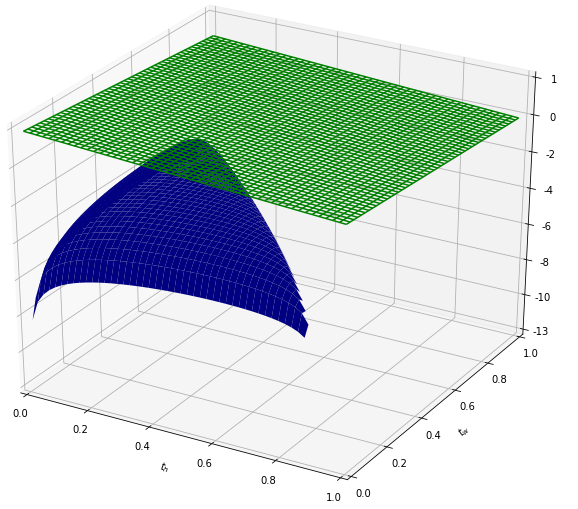
\includegraphics[width=\textwidth]{plotNumericalExample01.png}
%	\caption{The utility maximisation problem for $\alpha=T=0.1$ and $Q=1$}
%\end{figure}
%
%
%
%\begin{figure}[!ht]
%	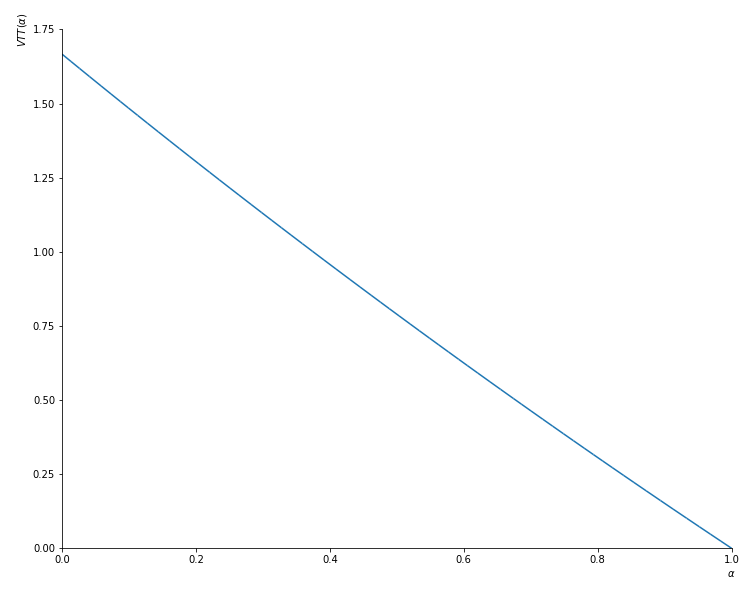
\includegraphics[width=\textwidth]{plotNumericalExample02.png}
%	\caption{The value of travel time variability as a function of $\alpha$}
%\end{figure}

\begin{figure}%
	\centering
	\subfloat[The objective and constraint funcitons for $\alpha=T=0.1$ and $Q=1$]{{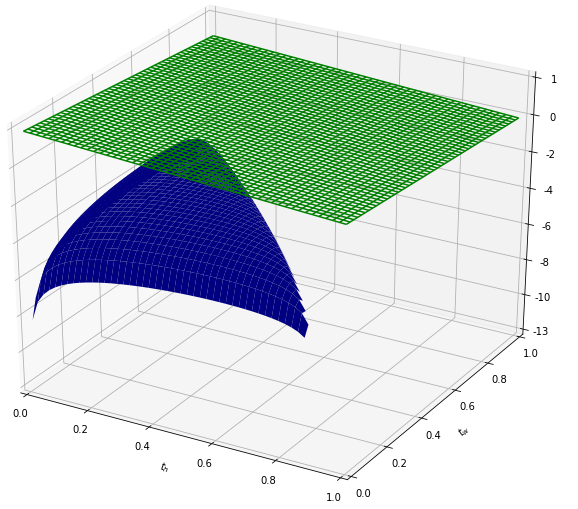
\includegraphics[width=0.48\textwidth]{plotNumericalExample01.png}}}%
	\quad
	\subfloat[The value of travel time as a function of $\alpha$]{{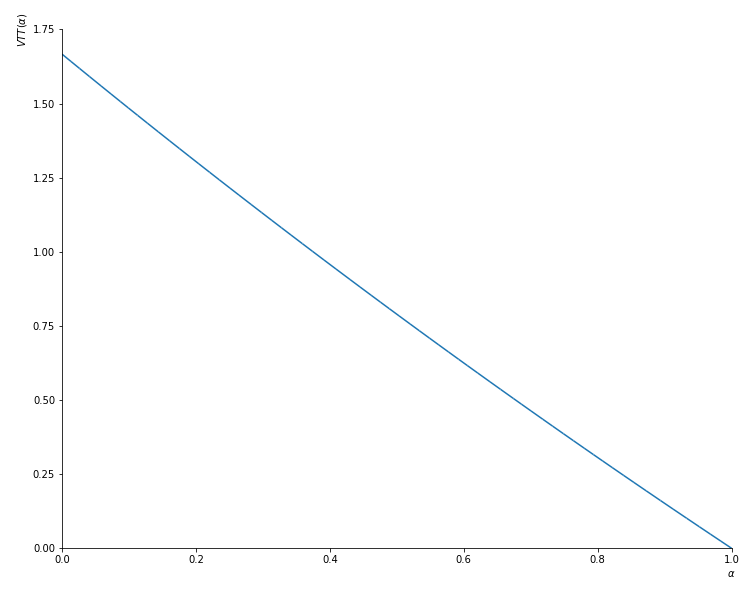
\includegraphics[width=0.48\textwidth]{plotNumericalExample02.png} }}%
	\caption{Some features of the optimum}%
	\label{fig:example}%
\end{figure}



% \begin{figure}[!ht]
% \centering
% 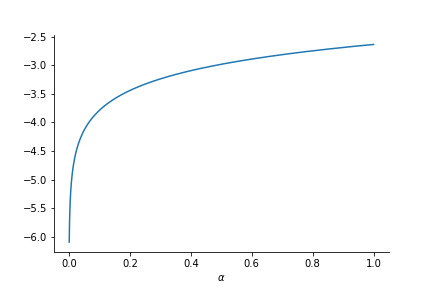
\includegraphics{uStarAlpha}
% \caption{Optimal utility as a function of $\alpha$}
% \end{figure}


\section{Allocation of time and the values of travel time and reliability with random travel time }

\subsection*{Optimal time allocation with random trip duration}

Suppose travel time $T$ is a random variable with a distribution bounded between $0$ and $Q$ \textit{such that the time constraint is never exceeded}.\footnote{The commuter takes the trip expecting that he or she will have some time at the destination to carry out the work-based activity. Hence, the travel time should be bounded within a reasonable limit for the trip to be taken. How can we put a bound to the distribution of travel time to take into account this?} We parametrise travel time in a convenient form $T=\mu+\sigma X$, where $\mu$ is its mean, $\sigma$ its standard deviation and $X$ is a standardised random variable with zero mean and unit variance and a probability density function $f\left(X\right)$.

Since utility depends on the unknown travel time, $T$, it is stochastic and hence the exact outcome for a given allocation of time cannot be determined before the trip. We assume the commuter allocates the total available time across different activities in view of a known travel time distribution. The choice of optimal time allocation is taken sequentially. Firstly, for a given travel travel and time assigned to the work-based activity, the commuter optimally allocates his or her time at home between the home-based and mobile activities. Once travel time is realised upon arrival at work, the commuter optimally allocates the remaining time between the work-based and mobile activities. We solve the utility maximisation problem by backward induction: Conditional on the information at the time of arrival at work, the commuter determines the optimal time to be assigned to the work-based activity given the realised travel time and the time devoted to the home-based and mobile activities. Then, the optimal time for the home-based activity is determined considering the distribution of travel times.

Upon arrival at the destination, the commuter has $Q-T-t_{d}$ time units to be allocated between the mobile and work-based activities.
As travel time is realised, the commuter faces no uncertainty and his/her problem amounts to:
\begin{align}
\begin{split}
\max_{t_{w}} \quad & U_{m}\left(Q - \left(1 - \alpha\right) \left(\mu + \sigma X\right) - t_{h} - t_{w}\right) + U_{w}\left(t_{w}\right) \\
\mbox{subject to } \,\, & t_{w} \leq Q-\mu-\sigma X-t_{d} \\
 & t_w \geq 0
\end{split}
\label{eq:secondStageProb}
\end{align}
The constraint indicates that the time that will be allocated to the work-based activity cannot exceed the total available time at the
destination. The Lagrangian of the maximisation problem will be%
\begin{equation*}
U_{m}\left(Q-\left(1-\alpha\right)\left(\mu+\sigma X\right)-t_{h}-t_{w}\right)+U_{w}\left(t_{w}\right)+\eta\left(Q-\mu-\sigma X-t_{d}-t_{w}\right),
\end{equation*}
with first-order conditions for an optimum being%
\begin{subequations}
\label{eq:tw_stage}
\begin{align}
U_{w}^{\prime}\left(t_{w}\right)-U_{m}^{\prime}\left(Q-\left(1-\alpha\right)\left(\mu+\sigma X\right)-t_{h}-t_{w}\right)-\eta & =0
\label{eq:stage2_wrt_tw}\\
\eta\left(Q-\mu-\sigma X-t_{d}-t_{w}\right) & =0\label{eq:stage2_compl}\\
\eta,t_{w} & \geq 0
\label{eq:stage2_nonnegative}
\end{align}
\end{subequations}
If the commuter has a non-binding constraint, then the optimal time assigned to the work-based activity, $\hat{t}_{w}$, will be that which equates the value of time assigned to the work-based and mobile activities. If however the commuter faces binding constraint, then all the time at the destination will be assigned to the work-based activity, hence $\hat{t}_{w}=Q-t_{d}-\mu-\sigma X$. In this case, the value of time assigned to the work-based activity will be higher than that allocated to the mobile activity. This is so since, if this was not the case, then the commuter will be better off allocating some of the time at the destination to the mobile activity. If there exists a pair $\left(\hat{t}_{w},\hat{\eta}\right)$ satisfying the first-order conditions in (\ref{eq:tw_stage}), then the optimal utility at this stage is\begin{equation*}
V\left(\hat{t}_{w};t_{h}, X\right)\equiv U_{m}\left(\hat{t}_{w}; t_{h}, X\right) + U_{w}\left(\hat{t}_{w}\right).
\end{equation*}
Note that, the time optimally assigned to the work-based activity, $\hat{t}_w(t_h)$, is a defined for a given time assigned to the home-based activity, $t_h$. Given the optimal allocation of time at work, the commuter will determine the optimal allocation of the total time at the origin between the home-based and mobile activities. This decision is made in light of the travel time distribution as the exact travel time is not known before the trip. The commuter's problem then is to choose the time to be assigned to the home-based activity in order to maximise expected utility:
\begin{align}
\begin{split}
\max_{t_{h}} \quad & E\left[U_{h}\left(t_{h}\right)+V\left(\hat{t}_{w};t_{h}, X\right)\right]\\
\mbox{subject to } \,\, & t_{h} \leq t_{d} \\
& t_h \geq 0
\end{split}
\label{eq:firstStageProblem}
\end{align}
where the expectation is over all possible values of the standardised travel time, $X$. The Lagrangian of the utility maximisation problem can be given as:
\begin{equation*}
E\left[U_{h}\left(t_{h}\right) + U_{m}\left(t_{h}, \hat{t}_{w}; X \right) + U_{w}\left(\hat{t}_{w}\right) + \phi\left(t_{h} - t_{d} \right)\right]
\end{equation*}
with first-order conditions
\begin{subequations}\label{eq:th_stage}
\begin{align}
E\left[U_{h}^{\prime}\left(t_{h}\right) - U_{m}^{\prime}\left(t_{h} ,\hat{t}_{w}; X\right) - \phi\right] & =0
\label{eq:stage1_wrt_th}\\
\phi,t_{h} & \geq 0
\label{eq:stage1_lambda}\\
\phi\left(t_{d}-t_{h}\right) & =0
\label{eq:stage1_lambdai_const}
\end{align}
\end{subequations}

An optimal allocation exists if there is a quartet $\left(\hat{t}_{h},\hat{t}_{w},\hat{\eta},\hat{\phi}\right)$ satisfying the conditions in (\ref{eq:tw_stage}) and (\ref{eq:th_stage}). The existence and uniqueness of such an optimum is given in the following theorem:
\begin{theorem}
\label{thm:existence_stochastic}
Suppose $0<T<Q$ and each utility component is increasing, strictly concave and twice-continuously differentiable. Then, there exists a unique optimal time allocation, $\left(\hat{t}_{h},\hat{t}_{w}\right)$, and multipliers $\hat{\eta}$ and $\hat{\phi}$ satisfying (\ref{eq:tw_stage}) and (\ref{eq:th_stage}).
\end{theorem}


\begin{proof}
We want to show the existence of a unique quartet $\left( \hat{t}_{h},\hat{t}_{w}, \hat{\eta},\hat{\phi}\right)$ such that $\left( \hat{t}_{w}, \hat{\eta}\right)$ solves \eqref{eq:secondStageProb} given $\left( \hat{t}_{h},\hat{\phi}\right)$ and $\left( \hat{t}_{h},\hat{\phi}\right)$ solves \eqref{eq:firstStageProblem} given $\left( \hat{t}_{w},\hat{\eta}\right)$. The existence of a unique solution for each problem is given by the proof of Theorem \ref{thm:optimum_det}. The same proof establishes the existence of a unique joint solution if $V\left(\hat{t}_{w};t_{h}\right)$ is strictly concave in $t_{h}$. Since $V$ is continuous in $t_{h}$, strict concavity follows if $\frac{\partial}{\partial t_{h}}\left(\frac{\partial V}{\partial t_{h}}\right) \leq 0$. To see if this is the case, twice differentiate $V$ to find that%
\begin{equation*}
\frac{\partial}{\partial t_{h}}\left(\frac{\partial V}{\partial t_{h}}\right) = U_{m}^{\prime\prime} \left(t_{h}, \hat{t}_{w}; X \right) \left( 1 + \frac{\partial\hat{t}_{w}}{\partial t_{h}}\right)
\end{equation*}
So, strict concavity holds if $\frac{\partial\hat{t}_{w}}{\partial t_{h}} > -1$. Differentiating \eqref{eq:stage2_wrt_tw} and manipulating, we see that  $\frac{\partial\hat{t}_{w}} {\partial t_{h}} \geq 0$ and hence $V$ is strictly concave.
\end{proof}


The commuter chooses an optimal departure time given the choice of optimal allocation. This choice depends on the status of the two constraints: If the commuter has binding constraints at both ends of the trip, then $\hat{t}_{w}=Q-t_{d}-\mu-\sigma X$ and the mobile activity will be carried out only while travelling, hence $\hat{t}_{m}=\alpha\left(\mu+\sigma X\right)$. In this case, the expected marginal utility of time in the mobile activity will be lower than that in the home-based or work-based activities. In addition, $\hat{t}_{h}=t_{d}$, hence the commuter will depart as soon as he/she spent the last minute of the time allocated to the home-based activity. This is also the case with binding constraint at home irrespective of the status of the constraint at work.

On the other hand, if both the constraints are non-binding, then the marginal expected utility of time will be equalised across the three activities. This is analogous to the case with deterministic travel time. In this case, the optimal departure time can be any moment between $\hat{t}_{h}$ and $Q-\hat{t}_{w}-\mu-\sigma X$.\footnote{Since the exact travel time is unknown before the trip, the optimal departure time may be determined based on a predicted travel time such as the mean, median or other features of the travel time distribution.} This is also the case if the constraint at home is non-binding irrespective of whether the constraint at work is binding.

If the commuter has binding constraint at work but non-binding constraint at home, i.e., $\eta>0$ and $\phi=0$, then optimality requires that the expected marginal utility of time in the work-based activity be higher than that in the mobile or home-based activities. In this case, the optimal departure time can be any moment between $\hat{t}_{h}$ and $Q-\hat{t}_{w}-\mu-\sigma X$. Conversely, in the case where the constraint at home is binding while that at work is not, the optimal departure time will be $\hat{t}_{h}$ units of time in the home-based activity, and the expected marginal utility of time in the home-based activity will be higher than that in the mobile or work-based activities.

The optimal expected utility:
\begin{equation*}
W\equiv E\left[U\left(\hat{t}_{h},\hat{t}_{w}; X\right)\right] = E\left[ U_{h}\left(\hat{t}_{h} \right) + U_{m}\left(\hat{t}_{h},\hat{t}_{w}; X\right) + U_{w}\left(\hat{t}_{w}\right)\right],
\end{equation*}
increases with the productivity of in-vehicle time, $\alpha$. Hence, as was the case with deterministic travel time, an improvement in the productivity of in-vehicle time is welfare improving.

% \subsection*{Example}

% \subsection*{The value of time and reliability with random travel time}

\subsection*{The value of travel time}

% The value of (mean) travel time equals the expected difference in the value of time assigned to the work-based activity and that assigned to the mobile activity:
% The value of reduced mean travel time is the difference in the expected value of time assigned to the work-based activity and the expected value of in-vehicle time:
The value of reduced mean travel time is the sum of the resource value of time at work and the expected marginal benefit from undertaking the mobile activity at home/work rather than in-vehicle:
\begin{align}
-\frac{\mathrm{d}W}{\mathrm{d}\mu} & = E\left[ \left( 1 - \alpha\right) U_m^{\prime} \left(\hat{t}_{h}, \hat{t}_{w}; X \right) \right] + \hat{\eta}
\label{eq:VOT_stochastic}
\end{align}
Substituting \eqref{eq:stage2_wrt_tw} in the above and rearranging, the value of travel time can be given by $E\left[ U_{w}^{\prime}\left( \hat{t}_{w} \right) - \alpha U_{m}^{\prime}\left(\hat{t}_{h}, \hat{t}_{w}; X\right)\right]$.  Notice that this is analogous to the expression for the value of travel time with deterministic travel time. Now, since travel time is uncertain, the the value of travel time is the \textit{expected} gain from using the reduced in-vehicle time for the work-based activity rather than for undertaking the mobile activity en route to work.

We now examine the value of travel time with respect to the productivity of in-vehicle time for commuters with and without binding time constraints. If in-vehicle time is fully productive, i.e., $\alpha=1$,  then the value of travel time for commuters with non-binding constraints equals zero\footnote{This may be similar to a finding where leisure ... } while those with binding constraints will have a positive value of travel time. This result is similar to the case with deterministic travel time and it indicates that ...

If the constraint at the destination is non-binding and travel time is fully productive, then the value of travel time will be zero. However, if the constraint is binding, then the value travel time will be positive even if travel time is fully productive. This result is similar to the case with deterministic travel time.

Since $E\left[U_{w}^{\prime}\left(\hat{t}_{w}\right)\right] \geq E\left[U_{m}^{\prime} \left( \hat{t}_{h}, \hat{t}_{w}; X\right)\right]$, then the value of travel time is non-negative.

\begin{prop}
The value of travel time declines with an exogenous improvement in the productivity of in-vehicle time if
\begin{enumerate}
\item the commuter has non-binding time constraints; or
\item the relative risk aversion of $U_m$ is less than or equal to unity should the constraints be binding.
\end{enumerate}
\end{prop}

\begin{proof}
Differentiating (\ref{eq:tw_stage}) and (\ref{eq:th_stage}) with respect to $\alpha$ and rearranging, we observe that $\frac{\partial\hat{t}_{h}}{\partial\alpha} \geq 0$ and $\frac{\partial\hat{t}_{w}}{\partial\alpha}\geq0$. In particular, if the constraints are non-binding, then $\frac{\partial\hat{\eta}}{\partial\alpha}=0 $ and
\begin{equation*}
\frac{\partial\left(-\frac{\mathrm{d}W}{\mathrm{d}\mu}\right)}{\partial\alpha} = E\left[\left(1-\alpha\right)  \left( \mu + \sigma X \right) \left(\frac{\prod_{i \in\left\{ h, m, w \right\}}U_{i}^{\prime\prime}\left(\hat{t}_{i}\right)}{\sum_{i\neq j}U_{i}^{\prime\prime}\left(\hat{t}_{i}\right)U_{j}^{\prime\prime}\left(\hat{t}_{j}\right)}\right)-U_{m}^{\prime}\left(\hat{t}_{h}, \hat{t}_{w}; X\right)\right] \leq 0
\end{equation*}
where the inequality follows since $0 \leq \alpha \leq 1$ and $U^{\prime\prime}_i < 0 < U^{\prime}_i$.  If the constraints are binding, then $\frac{\partial\hat{t}_{h}}{\partial\alpha}=\frac{\partial\hat{t}_{w}}{\partial\alpha}=0$, $\hat{t}_{m}=\alpha \mu + \sigma X$ and $\frac{\partial\hat{\eta}}{\partial\alpha}=-(\mu+\sigma X) U_{m}^{\prime\prime}\left(\alpha (\mu+\sigma X) \right)$. Therefore,
\begin{equation*}
\frac{\partial\left(-\frac{\mathrm{d}W}{\mathrm{d} \mu}\right)}{\partial\alpha}= E\left[-\alpha (\mu + \sigma X) U_{m}^{\prime\prime}\left(\alpha (\mu+\sigma X) \right)-U_{m}^{\prime}\left(\alpha (\mu+\sigma X) \right)\right] \leq 0
\end{equation*}
if $R_m \equiv \frac{-\alpha (\mu+\sigma X) U_m^{\prime\prime} \left(\alpha (\mu+\sigma X)\right)}{U_m^{\prime\prime} \left(\alpha (\mu+\sigma X)\right)} \leq 1$.
\end{proof}


The value of travel time depends on the difference in marginal value of time spent in performing the work-based activity and that undertaking the mobile activity while travelling. When the productivity of in-vehicle time increases, other things held constant, the difference in marginal value hence the VTT declines. However, the optimal allocation too could change and when it does, this difference in value of travel time can become larger or smaller depending on whether $T < \frac{\partial \hat{t}_h}{\partial \alpha}$. Accordingly, if $\frac{\partial \hat{t}_h}{\partial \alpha} > T$, then the VTT declines with the productivity of in-vehicle time. Otherwise, $\frac{\partial\left( -\frac{\mathrm{d}W }{\mathrm{d}\mu} \right)}{\partial\alpha} \leq 0$ requires that the coefficient of absolute risk aversion of $U_m$ be less than $\left( \alpha \left(T - \frac{\hat{t}_h}{\partial \alpha} \right) \right)^{-1}$


%{\color{red}
%\begin{enumerate}
%    \item The VTT depends on the difference of MU(work) and alpha * MU(M), so when alpha increases:
%    \begin{itemize}
%        \item For a given time allocation, the VTT declines with the productivity of in-vehicle time since the productivity gap in performing the mobile activity at home/work and in-vehicle declines.
%        \item But other things may not remain constant. In fact, if some or both the constraints are non-binding, then a change in productivity of in-vehicle time could lead to a new optimum. The VTT at the new optimum will be lower only if the $\vartheta \leq 1$ or $\frac{\partial \hat{t}_{m}}{\partial \alpha} \leq T$
%    \end{itemize}
%\end{enumerate}
%}
%
%Note the following:
%\begin{enumerate}
%\item If both constraints are binding, then $\frac{\partial\hat{t}_{w}}{\partial\alpha} = T$ , which cannot be negative. Thus, the claim holds only if $\vartheta < 1$.
%\item If either constraint is binding, the inequality in the above claim holds only if the accompanying change in $\left(\hat{t}_w,\hat{t}_h\right)$ exceeds the total travel duration.
%\item If both constraints are non-binding, then barring the size of $\vartheta$, the above claim holds if and only if $\frac{\partial \left(\hat{t}_w + \hat{t}_h \right)} {\partial\alpha} > T$.
%\item All the above is so since the VTT depends on the difference in the productivity of performing the mobile activity at home/work compared to while travelling. When $\alpha$ increases, given the optimal allocation, the gap in productivity hence the VTT declines. However, the optimal allocation too could change and when it does, this   gap can be larger or smaller
%\end{enumerate}


\subsection*{The value of reliability}

The value of reliability in our model is:
\begin{align*}
-\frac{\mathrm{d}W}{\mathrm{d}\sigma} & = E\left[\left( 1 - \alpha \right) X U_{m}^{\prime} \left(\hat{t}_{h}, \hat{t}_{w}; X\right)\right],
\end{align*} %
which is proportional to $1-\alpha$. As stated in the following lemma, the value of reliability is non-negative implying that the commuter is willing-to-pay a certain amount for a reduction in the degree of travel time variability.

\begin{lemma}
An exogenous reduction in travel time variability is beneficial to the commuter, i.e., the value of reliability is non-negative.
\end{lemma}

\begin{proof}
Let $ v_1 $ and $v_2$ respectively denote the value of $U_{m}^{\prime}\left(\hat{t}_{h}, \hat{t}_{w}; X\right)$ for $ X > 0$ and $X \leq 0$, where $v_{1}$ and $v_{2}$ are positive constants with $v_{1}\geq v_{2}$ since $\frac{\partial U_{m}^{\prime} \left(\hat{t}_{m}\right)}{\partial X} \geq 0$. Using this, the value of reliability can be given as
\begin{align*}
-\frac{\mathrm{d}W}{\mathrm{d}\sigma} & = E\left[\left(1-\alpha\right) X U_{m}^{\prime} \left(\hat{t}_{h}, \hat{t}_{w}; X\right)\vert X>0\right]  + E\left[\left( 1 - \alpha \right) X U_{m}^{\prime}\left( \hat{t}_{h}, \hat{t}_{w}; X\right) \vert X\leq 0 \right] \\
 & = E\left[\left( 1 - \alpha \right) v_{1} X \vert X > 0 \right] + E\left[\left( 1 - \alpha \right) v_{2} X \vert X \leq 0 \right]
 \end{align*}%
Noting that $E\left[X\right]=0$ such that $E\left[X \vert X \leq 0 \right] = -E\left[ X \vert X > 0 \right]$, we have%
\begin{align*}
- \frac{\mathrm{d}W}{\mathrm{d}\sigma} & = \left(1-\alpha\right) v_{1} E\left[X\vert X > 0 \right] + \left(1-\alpha \right) v_{2} E\left[X \vert X\leq0\right]\\
 & =\left(1-\alpha\right)v_{1}E\left[X\vert X>0\right]-\left(1-\alpha\right)v_{2}E\left[X\vert X>0\right]\\
 & =\left(1-\alpha\right)\left(v_{1}-v_{2}\right)E\left[X\vert X>0\right]\\
 & \geq0
\end{align*}
where the inequality follows since $v_{1}\geq v_{2}$ and $E\left[X\vert X>0\right] > 0$. Therefore, the value of reliability is non-negative.
\end{proof}

Notice that the value of reliability equals the weighted mean of gains from undertaking the mobile activity at work instead of while travelling. Thus, if in-vehicle time is as productive as time at work, i.e., $\alpha=1$, then the commuter does not gain by using the reduced travel time to carry out the mobile activity at work. Hence, the value of reliability will be zero if in-vehicle time is fully productive. This is new compared to previous literature \citep{Small1982SchedulingConsumerActivities,FosgerauEngelson2011ValueTravelTime,FosgerauKarlstroem2010ValueReliability} who


\todo[inline]{Compare the value of reliability in our model against that in \citet{FosgerauEngelson2011ValueTravelTime}, where $ \beta, \gamma <0 $ shall be assumed so their result can be comparable to ours}

\todo[inline]{Note: The following need revision as it does not hold in general, and it proved to be difficult to come up with a conditon that ensures the inequality holds}

\begin{prop}
	WRONG !!!
The value of reliability declines with an exogenous increase in the productivity of in-vehicle time provided that both constraints are binding or non-binding.
\end{prop}

\begin{proof}
If both constraints are non-binding, then $\hat{\eta}=\hat{\phi}=0$ and hence
\begin{align*}
\frac{\partial\left(-\frac{\mathrm{d}W}{\mathrm{d}\sigma}\right)}{\partial\alpha} &= E\left[\left(\left(1-\alpha\right)\left(\mu+\sigma X\right) \frac{\prod_{i \in \left\{ h,w,m\right\}  }U_{i}^{\prime\prime}\left(\hat{t}_{i}\right)}{\sum_{i\neq j}U_{i}^{\prime\prime}\left(\hat{t}_{i}\right)U_{j}^{\prime\prime}\left(\hat{t}_{j}\right)}-U_{m}^{\prime}\left(\hat{t}_{m}\right)\right)X\right] \leq 0
\end{align*}
where the inequality follows since the expression in parenthesis is negative. If the constraints are binding, then $\frac{\partial\hat{t}_{h}}{\partial\alpha}=\frac{\partial\hat{t}_{w}}{\partial\alpha}=0$, and hence $\frac{\partial\hat{t}_{m}}{\partial\alpha}=\mu+\sigma X$ and
\begin{equation*}
\frac{\partial\left(-\frac{\mathrm{d}W}{\mathrm{d}\sigma}\right)}{\partial\alpha}=E\left[\left(\left(1-\alpha\right)\left(\mu+\sigma X\right)U_{m}^{\prime\prime}\left(\hat{t}_{m}\right)-U_{m}^{\prime}\left(\hat{t}_{m}\right)\right)X\right] \leq 0.
\end{equation*}
Therefore, $\frac{\partial\left(-\frac{\mathrm{d}W}{\mathrm{d}\sigma}\right)}{\partial\alpha} \leq 0 $ irrespective of whether the constraints are binding.
\end{proof}

An increase in the productivity of in-vehicle time reduces the $\left(1-\alpha\right)$ and hence also the value of reliability, but its effect through $t_{m}$ depends on if and how much the optimal allocation of time changes due to a change in $\alpha$. With binding time constraints at both ends of the trip, $\frac{\partial t_{m}}{\partial\alpha}=\mu+\sigma X>0$ since the time optimally allocated to the home-based and work-based activities will remain unchanged. Thus, the value of reliability declines with the productivity of in-vehicle time irrespective of the value of $\frac{\partial t_{m}}{\partial\alpha}$. However, when one or both constraints are inactive, a change in productivity of in-vehicle time also affects the value of reliability through its effect on the optimal allocation of time. Accordingly, an increase in $\alpha$ increases $t_{h}$ or $t_{w}$ or both. As a result, the value of reliability declines with the productivity of in-vehicle time only if the sum of the change in time devoted to the home-based and work-based activities does not exceed the travel time, i.e., $\frac{\partial\hat{t}_{h}}{\partial\alpha}+\frac{\partial\hat{t}_{w}}{\partial\alpha}\leq\mu+\sigma X$.


\section{Discussion and conclusion}

The model examines the optimal allocation of time among different activities and the valuation of travel time and reliability with self-driving cars. It analyses how the values of travel time and reliability changes with increased productivity of in-vehicle time.

\clearpage

% \bibliographystyle{authordate1}
\bibliographystyle{chicago}
\bibliography{references}

\end{document}
